


\section{MOTIVATION}
Currently the main channel for job seekers are online job finding web sites, like indeed or monster, etc, that make the job finding process easier and decrease the recruitment time. But most such web sites only allow users to use key word to search the jobs, which makes job searching as a tedious and blind task. For example, I used keywords ``Java'' to search jobs with location restriction Mountain View, CA on the job searching site indeed.com, the web site returned about 7,000 jobs (Figure~\ref{fig:Indeed}). The number of results of job searching is huge, but un-ranked, so the job seeker has to review every job description. Since no one has enough time to read all the jobs in the searching result, the actual quality of job searching service is low. This is a classic problem of information overflow.


\begin{figure}[htbp]
  \centering
  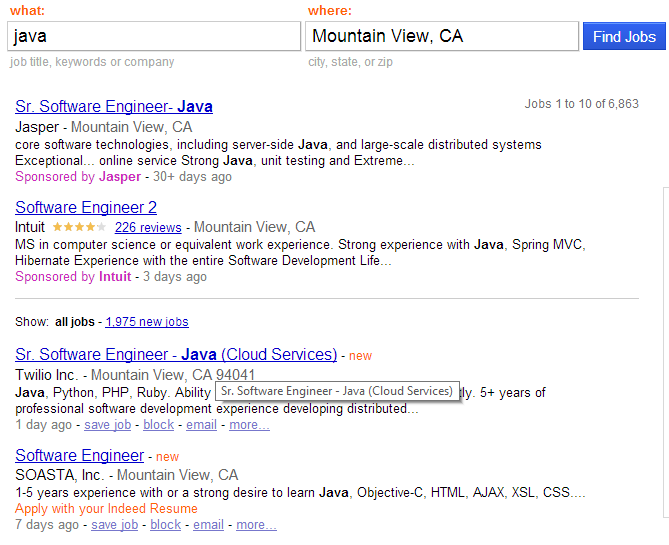
\includegraphics[scale=0.4]{images/indeed1.png}
  \caption{Search result of Indeed}
  \label{fig:Indeed}
\end{figure}

The reason for such result is because current job searching web sites use the same information retrieval technology like ``Inverted index'' \cite{zobel2006inverted} as the common search engines, which just use keywords to map all the stored documents. Modern search engines all have some ranking algorithms to sort the searching result, like page rank \cite{page1999pagerank}, so the top results are the most related ones. But such algorithms are unavailable to the job searching systems, because the criteria  of how to rank the job searching result is very personalized. A great job opening for one job seeker maybe looks not good to the other, because the goodness of a job to a specular job seeker heavily depend on his personal background, like his education or professional experience etc.

Since the people's resumes contain the most important background information, we believe the content of the resume could be used to rank the job openings. My proposal is to create a web system which could use the resumes of job seekers to find the jobs that match their profiles best. The main idea is to calculate the similarity between the candidate model and job models, which should be generated from resumes and job descriptions. I want to transfer the job searching task from key word searching to job and resume models matching. The matching result should be sorted by the matching score, higher matching score means a better matching. The matching algorithm not only help job seekers find the appreciate job opening, but also offer priority to them.~\cite{gueutal2006brave}  The job with higher matching score means the job is more appropriate to the job seeker, and if he applies to the job, the chances of getting the interview call will be higher as well. Figure~\ref{fig:Matching} shows how this approach works.


\begin{figure}[htbp]
  \centering
  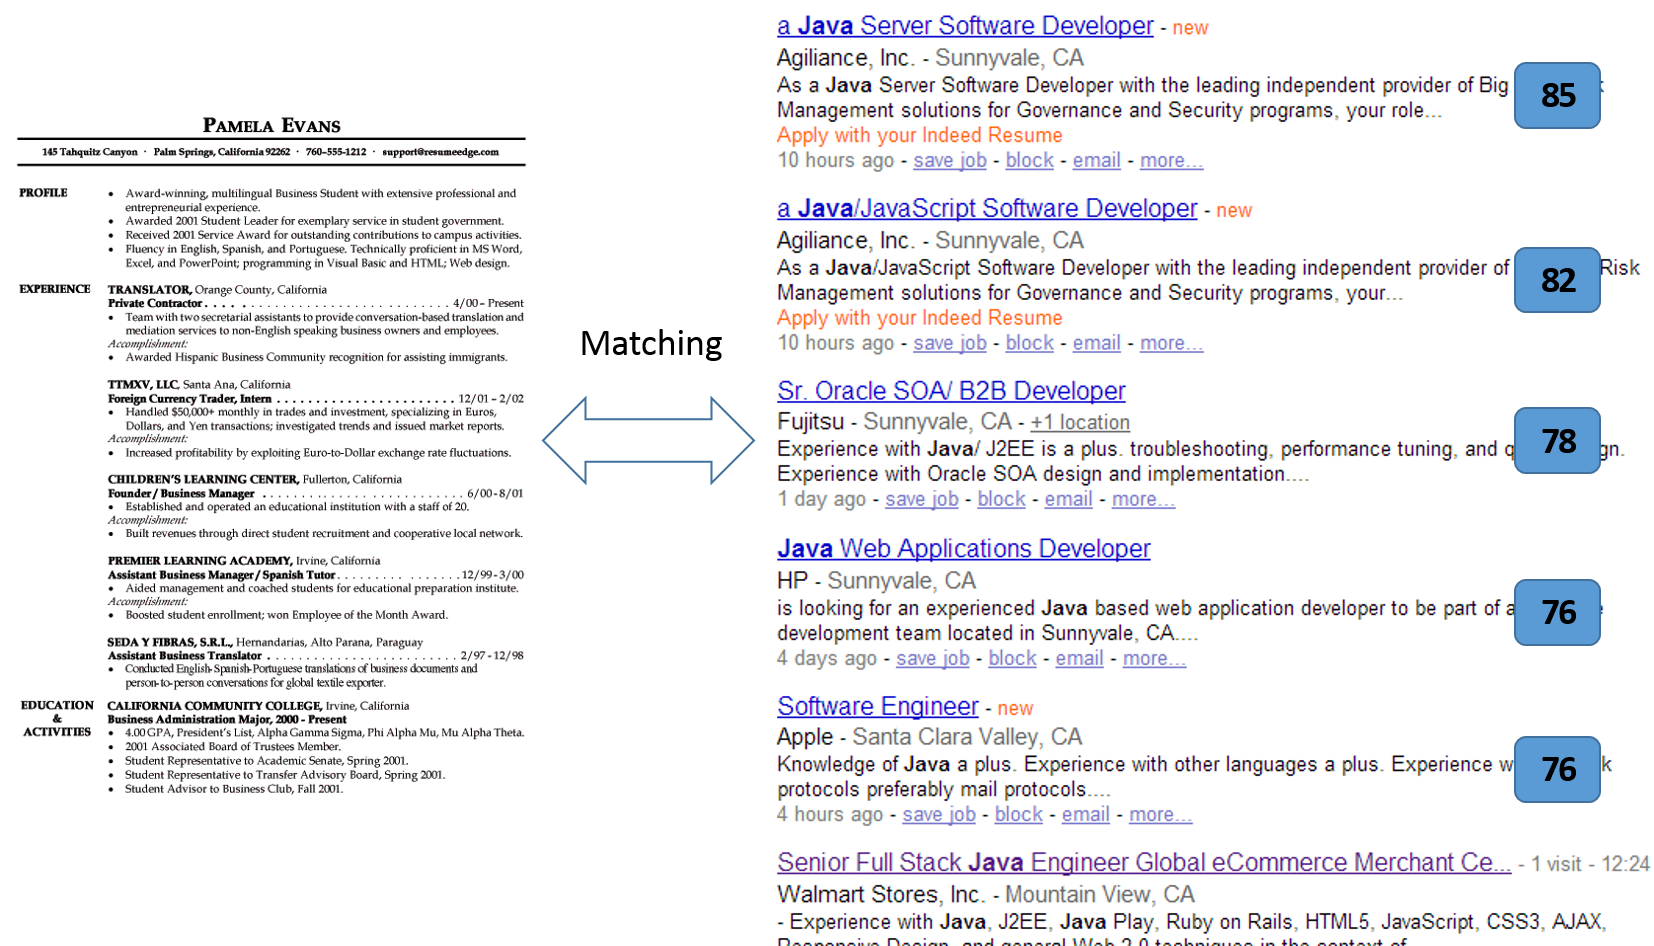
\includegraphics[scale=0.5]{images/matching.png}
  \caption{Matching the job opening with Resume}
  \label{fig:Matching}
\end{figure}

\section{PREVIOUS WORK}

Some scholars found that current Boolean search and filtering techniques cannot satisfy the complexity of candidate-job matching requirement.~\cite{malinowski2006matching} They hope the system could understand the job requirement, determine which requirements are mandatory and which are optional but preferable. So they moved to use recommender systems technique to address the problem of information overflow.

\subsection{Job Recommender System}

Job searching is not a new topic in information retrieval, which has been the focus of some commercial job finding web sites and research papers. Usually scholars called them Job Recommender System (JRS), because most of them used technologies from recommender systems. Wei et al. classified Recommender Systems into four categories~\cite{wei2007survey}: Collaborative Filtering, Content-based filtering, Knowledge-based and Hybrid approaches. Some of these techniques had been applied into JRS; Zheng et al. ~\cite{siting2012job} and AlOtaibi et al.~\cite{al2012survey} summarized the categories of existing online recruiting platforms and listed the advantages and disadvantages of technical approaches in different JRSs. The categories include:

\begin{enumerate}
    \item Content-based Recommendation (CBR) The principle of a content-based recommendation is to suggest items that have similar content information to the corresponding users, like Prospect \cite{singh2010prospect}.

    \item Collaborative Filtering Recommendation (CFR) Collaborative filtering recommendation, which finds  similar  users  who have  the same taste with the target user and recommends items based on what the similar users, like CASPER~\cite{rafter2000personalised}.

    \item Knowledge-based Recommendation (KBR) In the knowledge-based recommendation, rules and patterns obtained from the functional knowledge of how a specific item  meets the requirement of a particular user, are used for recommending items, like  Proactive~\cite{lee2007fighting}.

\end{enumerate}

There are two main challenges in Content-Based Recommendation Systems: One is how to extract the information from the job descriptions and job seekers' resumes, the other is how to calculate similarity of them.


\subsection{Information Extraction}
One important the problem of this system is how to build the models from Job Description and Resume. The first step of the model generating is information extraction. Both resumes and job descriptions are written in natural language, so we need to extract information from such un-structured or semi-structured data source, and transfer them to some designed structure.

Yu et al.~\cite{yu2005resume} used a cascaded information extraction (IE) framework to get the detailed information from the job seeker��s resume. In the first stage, the Hidden Markov Model (HMM) is used to segment the resume into consecutive blocks. Based on the result, an SVM model is used to obtain the detailed information in the certain block, the information includes: name, address, education etc.

 Celik Duygua and Elci Atilla proposed an Ontology-based R��sum�� Parser (ORP) ~\cite{ccelik2013ontology}, which uses ontology to assistant the information extraction process. The system process the resume in following steps: convert the resume files into plain text, separate the text into  some segments, use Ontology Knowledge Base to find the concepts in the sentences, normalize all the terms, at last the system will classify the sentences to get the wanted terms.

\subsection{Matching Algorithms}

Lu et al~\cite{lu2013recommender}. used latent Semantic Analysis(LSA) to calculate similarities between jobs and candidates, but they only selected two factors ``interest'' and ``education''  to compare candidates. Xing et al. ~\cite{yi2007matching} used Structured Relevance Models (SRM) to  match resumes and jobs.

The Ontology technics had also been used in some JRSs, which had been well studied by  Shvaiko and Euzenat in \cite{shvaiko2013ontology}.  Proactive~\cite{lee2007fighting} used two kinds of ontology, job category and the company information. The system used ontology checker to classify the job information, stored the domain knowledge and calculated the weight value in recommendations.

Kumaran et al~\cite{kumaran2013towards} also used ontology to calculate the similarity between job criteria and candidates's resume in their system~\cite{kumaran2013towards}. The similarity equation they used are:
$$ M\left ( i_1, i_2 \right ) = \frac{\sum_{k=1}^{n} Sim\left (p_{k}^{i1},  p_{k}^{i2} \right ) * W_{k}^{i2}}{\sum_{k=1}^{n} W_{k}^{i2}}  $$
The similarity function $Sim(p_1, p_2)$ is defined as follows:
$$ Sim(p1, p2) = \begin{Bmatrix}
1, & if~similarity~of~p1~and~p2 \geqslant t\\
0, & otherwise
\end{Bmatrix} $$

Fazel \cite{fazel2009semantic} used a hybrid approach to matching job seekers and job postings, which takes advantage of the benefits of both logic-based and ontology-based matching. In his paper the description logics (DL) are used to represent the candidate and job opening, and the ontology is used to organize the skills in a skill taxonomy. He gave an equation to calculate the matching degree:
$$ sim\left(P ,j \right) = \sum x_{ij} \times u(ds_i) $$

where, $x_{ji}$ is the Boolean variable indicating whether desire i is satisfied by applicant $A_{j}$ in the set of all qualified applications.

Liu and Dew~\cite{liu2004using} used RDF to represent and store the expertise of experts , and a RDF-based Expertise Matcher could retrieves the experts whose expertise include the required concept.

\section{METHODOLOGY}

\subsection{Contribution}

There are some scholars noticed that the accuracy and completeness of information extracted from resumes and job descriptions have great influence on the final recommend results. Some of them used natural language processing techniques to extract information fields from job seekers' resumes.  But to the job description, very little work had been done, since most such systems were built for big companies to help them select applicants. So in my research work, I will construct a job description extractor.

The other contribution of the research is to a better domain specific ontology.  Even some systems used ontology to calculate the similarity between job and resume, but the ontology they build are relatively simple and rough, especially in skills part, like foreign language, IT skill. Such simple ontology cannot be applied in real situations, because the loose criteria will return huge matched results as well. So in this research I hope to build a more detailed ontology for IT jobs, which could include more and detailed IT skills, like some special databases, development frameworks, and special knowledge.

I hope with such improvement, the recommending result of the system will be more accurate, and the system could be more useful to the job seekers.

\subsection{System Overview}
The system will use rule based information extraction techniques to parse the job description and resume, and get information such as skill, specialties, and background. The information will be used to create the model of job description and job seeker.  Ontology will be used to construct the knowledge base, which will include the taxonomy and rules, to support resume-job matching.

The model of candidates will include their specialties, working experience, and education background, all of them should be extracted from the resumes. The job model will be extracted from job description, the information will include: company name, location, job title, education requirement, skill requirements and working experiences etc. When a job seeker searches the jobs by his resume, the system will calculate the similarity between the candidate model and the job models, give every job model a similarity score.

In the initial phase I will only focus on the positions of IT job, because IT jobs have a special character,  skill set oriented, which means the person that the company wants to hire must have some special skills and knowledge, like some programming languages, databases or software etc.

User��s personal preference should be considered as well. In the previous user survey, some factors will impact a lot on the user��s expectation of good jobs, such factors include: location, the reputation of the company, the salary etc. These factors will be treated as weight factors in the job matching algorithm.

Figure ~\ref{fig:Pipeline} shows the architecture of the whole system, which include such modules:

\begin{enumerate}
    \item The web crawler could search and download all new IT job opening web pages  from indeed.com everyday.
    \item The job parser could parse the job opening web page, extract the information and create the job model.
    \item Resume Parser is much like the Job parser, it will parse the resume and create the candidate model.
    \item All the job models will be stored in the Job Description database.
    \item When user makes a query request, the ontology matcher will calculate the matching score of each job, return the jobs ranked by their scores.
\end{enumerate}

\begin{figure}[htbp]
  \centering
  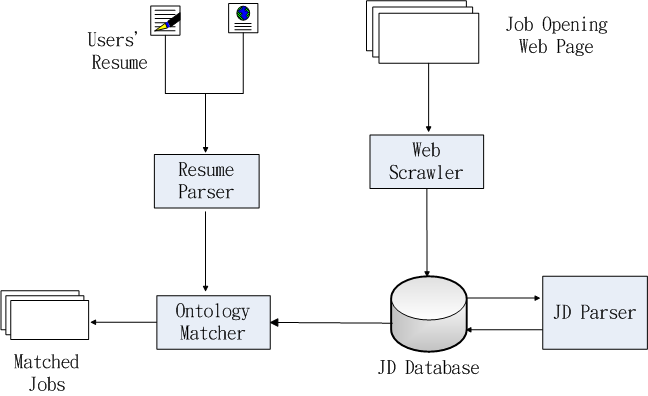
\includegraphics[scale=0.5]{images/arch.png}
  \caption{System Architecture}
  \label{fig:arch}
\end{figure}


\subsection{Information Extraction}
One important problem of this system is how to extract models from Job Descriptions and Resumes.
In Nature Language Processing, especially in Information Extraction, pipeline is a well adopted architecture~\cite{sarawagi2008information}. This architecture will also be used in this system to extract models of job openings and candidate's resumes. The system will process the job opening in the following steps, which is shown in Figure~\ref{fig:Pipeline}:

\begin{enumerate}
    \item The HTML parser will parse the job description web pages that are obtained from web crawler. It will get the HTML element that contains the main content of the job description.
    \item The segment module will separate the job description into paragraphs according to HTML tags at first, then separate each paragraph into sentences.
    \item The sentences will be tokenized as string array, and sent to the Classification module. Classification module will determine the category of the sentence, and mark the category of the sentence.
    \item The preprocessing module will delete unreadable characters, normalize some spelling tokens in the sentence.
    \item The annotation module will annotate the tokens with sematic and ontology labels. The sentences will be transferred to multi-layered data structure.
    \item The layered sentences will be matched with pre-defined patterns. If any pattern could be matched, the ontology information will be stored in the job model.
    \item After every sentence has be processed in the pipeline, the job model will be stored into database.
\end{enumerate}


\begin{figure}[htbp]
  \centering
  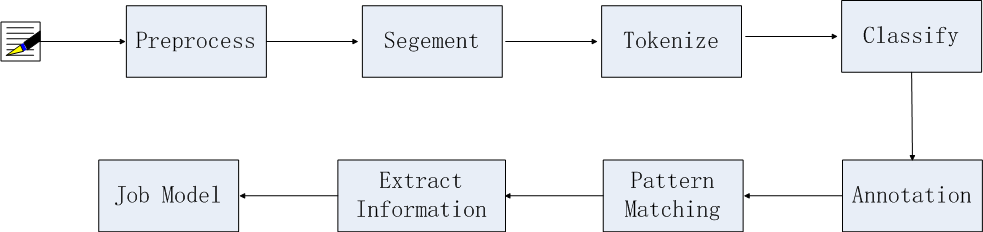
\includegraphics[scale=0.4]{images/pipeline.png}
  \caption{Job Description Process Pipeline}
  \label{fig:Pipeline}
\end{figure}

\subsection{Ontology Similarity}

We notice that simple keyword of skill name matching is far from enough, because job description and resume are both written in human language, even the same concepts, they could be written in different ways. For example, Table~\ref{tab:resume_jd}  is part of the resume of a job seeker, and part of a job description:

\begin{table}[ht]
\caption{Resume and Job Description} % title of Table
\centering % used for centering table
\begin{tabular}{ | p{8cm} | p{7cm} | }
 \hline
   \textbf{Part of Resume}                 &   \textbf{Part of Job Description}   \\ \hline

    B.S. degree in computer science \newline
    5+ years Java, \newline
    2+ year   C++  \newline
    Some experience in Oracle database \newline
    Other experience like: \newline
    Hibernate, JBOSS, JUnit, Tomcat etc.
  &
  BS degree above   \newline
  4+ years Java  \newline
  Some experience of Python   \newline
    Mysql, MS-SQL   \newline
    Java web application Server   \newline
    OOA/OOD   \\
 \hline
\end{tabular}
\label{tab:resume_jd} % is used to refer this table in the text
\end{table}

If just looking at the text, we can find the resume has few common words with the job description.  But from the view of an experienced engineer, the candidate is pretty matching the job. Because relational databases like Oracle and Mysql are very similar, OOA/OOD is the same meaning of many years of Java and C++ experience, and Tomcat and JBOSS are two Java web application servers.  If we use key word matching, the system won't give a good matching result in this very common situation. So when design the new ontology matching algorithm, we have such considerations:

\begin{enumerate}
    \item How to normalize the same concept with different names or spelling
    \item If one concept in the job description, but there is no the same one in the resume, how to calculate the similarity between its related concepts.
    \item If one concept in the job description has multiple similar concepts in the resume, how to summarize total similarity of them.
    \item When calculating the similarity between resume and job description, how to give weights to each concepts.
\end{enumerate}


\section{SYSTEM FEATURES}

The system should include such features:

\begin{enumerate}
    \item User could import his resume in different formats, like txt, doc and pdf.
    \item User could search jobs by his resume. The search result will be sorted by the matching scores.
    \item User could set their searching preference, like location, company type, reputation, salary level, etc.
    \item The system should be able to change the parameters of the matching algorithm adaptively according to the record of user's preference
    \item The user could set multiple searching agents, each one of which is a composition of different preferences, like one for remote location with high salary, another for local company with low salary.
\end{enumerate}


\section{EVALUATION}
To evaluate the system, some measures will be used. We also proposed two evaluation method: Pre-collected Data and User's direct experience.

\subsection{Basic measures of the system}

In traditional information retrieval system, some measures are widely used~\cite{manning2008introduction}. These measures include:

\begin{enumerate}
    \item Precision ($P$) is the fraction of retrieved documents that are relevant .
       $$  Precision =  \frac{ \#(releveant~items~ retrieved)}{ \#(retrieved~items)}$$
    \item Recall ($R$) is the fraction of relevant documents that are retrieved.
       $$  Recall =  \frac{ \#(releveant~items~ retrieved)}{ \#(releveant~items)}$$
    \item $F measure$ ($F_1 score$) trades off precision versus recall.
       $$ F_1 = 2 \cdot \frac{ Precision \cdot Recall}{ Precision + Recall } $$
    \item Since the results are ranked, $ Normalized~Discounted~Cumulative~Gain ( NDCG )$ will be an important measure to evaluate the ranked retrieval results. For a set of queries $Q$, let $R(j,d)$ be the relevance score assessors gave to document $d$ for query $j$.
       $$ NDCG(Q,k) = \frac {1}{|Q|} \sum_{j=1}^{|Q|}{Z_{kj}} \sum_{m=1}^{k} \frac{2^{R(j,m)} - 1}{ \log_2(1+m)} $$
where $Z_{kj}$ is a normalization factor calculated to make it so that a perfect ranking's NDCG at $k$ for query $j$ is 1. For queries for which $k' < k$ documents are retrieved, the last summation is done up to $k'$.

\end{enumerate}

\subsection{Pre-collected Data}

Some resumes will be pre-collected, and some their matched jobs will be found manually. These jobs will be put into the job database with some other unrelated jobs.  When searching the jobs with the resume, we can get precision, recall and F measure of the system. With ranking positions of the searching results we could calculate the NDCG measure.

\subsection{User Study}
Users will be asked to use both the system and current job finding web site. We can compare some factors to evaluate the system, such as:
\begin{enumerate}
    \item The time consumed to find satisfying jobs.
    \item The satisfaction of search results.
    \item The user subjective experience with the both systems.
\end{enumerate}


\section{TIME TABLE}
\begin{center}
\begin{tabular}{ |c|p{1cm}|p{1cm}|p{1cm}|p{1cm}|p{1cm}|p{1cm}| }
 \hline
  Content                 & May              & Jun             & Jul              & Aug             & Sep             & Oct  \\ \hline
  Literature Review       & \cellcolor{red}  & \cellcolor{red} &                  &                 &                 &      \\ \hline
  Data Collection         &                  & \cellcolor{red} & \cellcolor{red}  &                 &                 &      \\ \hline
  Requirement Analysis    &                  &                 & \cellcolor{red}  &                 &                 &      \\ \hline
  Implementation          &                  &                 &                  & \cellcolor{red} &                 &      \\ \hline
  Evaluation and Analysis &                  &                 &                  &                 & \cellcolor{red} &   \\ \hline
  Writing and Wrap Up     &                  &                 &                  &      & \cellcolor{red} & \cellcolor{red}     \\ \hline
  Defending               &                  &                 &                  &                 &     &  \cellcolor{red}    \\ \hline


 \hline
\end{tabular}
\end{center}

\section{CONCLUSION}

In this proposal I proposed a personalized job-resume matching system, which could help job seeker to find appropriate IT jobs more easily.  To improve the accuracy of the system, I want to construct on a job description extractor to retrieve information from job description, and want to build a domain specific ontology. In the system, job descriptions and resumes will be processed by pipeline; and a finite automated tool will be used to extract the model of them. The job descriptions will be matched the user's resume, the result will be sorted by the ontology similarity. Since the most appreciate jobs will be returned in front of other jobs, the users of the system could get better result than current job finding website. 
